\documentclass[noauthor,nooutcomes,handout,hints]{ximera}
\graphicspath{  
{./}
{./whoAreYou/}
{./drawingWithTheTurtle/}
{./bisectionMethod/}
{./circles/}
{./anglesAndRightTriangles/}
{./lawOfSines/}
{./lawOfCosines/}
{./plotter/}
{./staircases/}
{./pitch/}
{./qualityControl/}
{./symmetry/}
{./nGonBlock/}
}


%% page layout
\usepackage[cm,headings]{fullpage}
\raggedright
\setlength\headheight{13.6pt}


%% fonts
\usepackage{euler}

\usepackage{FiraMono}
\renewcommand\familydefault{\ttdefault} 
\usepackage[defaultmathsizes]{mathastext}
\usepackage[htt]{hyphenat}

\usepackage[T1]{fontenc}
\usepackage[scaled=1]{FiraSans}

%\usepackage{wedn}
\usepackage{pbsi} %% Answer font


\usepackage{cancel} %% strike through in pitch/pitch.tex


%% \usepackage{ulem} %% 
%% \renewcommand{\ULthickness}{2pt}% changes underline thickness

\tikzset{>=stealth}

\usepackage{adjustbox}

\setcounter{titlenumber}{-1}

%% journal style
\makeatletter
\newcommand\journalstyle{%
  \def\activitystyle{activity-chapter}
  \def\maketitle{%
    \addtocounter{titlenumber}{1}%
                {\flushleft\small\sffamily\bfseries\@pretitle\par\vspace{-1.5em}}%
                {\flushleft\LARGE\sffamily\bfseries\thetitlenumber\hspace{1em}\@title \par }%
                {\vskip .6em\noindent\textit\theabstract\setcounter{question}{0}\setcounter{sectiontitlenumber}{0}}%
                    \par\vspace{2em}
                    \phantomsection\addcontentsline{toc}{section}{\thetitlenumber\hspace{1em}\textbf{\@title}}%
                     }}
\makeatother



%% thm like environments
\let\question\relax
\let\endquestion\relax

\newtheoremstyle{QuestionStyle}{\topsep}{\topsep}%%% space between body and thm
		{}                      %%% Thm body font
		{}                              %%% Indent amount (empty = no indent)
		{\bfseries}            %%% Thm head font
		{)}                              %%% Punctuation after thm head
		{ }                           %%% Space after thm head
		{\thmnumber{#2}\thmnote{ \bfseries(#3)}}%%% Thm head spec
\theoremstyle{QuestionStyle}
\newtheorem{question}{}



\let\freeResponse\relax
\let\endfreeResponse\relax

%% \newtheoremstyle{ResponseStyle}{\topsep}{\topsep}%%% space between body and thm
%% 		{\wedn\bfseries}                      %%% Thm body font
%% 		{}                              %%% Indent amount (empty = no indent)
%% 		{\wedn\bfseries}            %%% Thm head font
%% 		{}                              %%% Punctuation after thm head
%% 		{3ex}                           %%% Space after thm head
%% 		{\underline{\underline{\thmname{#1}}}}%%% Thm head spec
%% \theoremstyle{ResponseStyle}

\usepackage[tikz]{mdframed}
\mdfdefinestyle{ResponseStyle}{leftmargin=1cm,linecolor=black,roundcorner=5pt,
, font=\bsifamily,}%font=\wedn\bfseries\upshape,}


\ifhandout
\NewEnviron{freeResponse}{}
\else
%\newtheorem{freeResponse}{Response:}
\newenvironment{freeResponse}{\begin{mdframed}[style=ResponseStyle]}{\end{mdframed}}
\fi



%% attempting to automate outcomes.

%% \newwrite\outcomefile
%%   \immediate\openout\outcomefile=\jobname.oc
%% \renewcommand{\outcome}[1]{\edef\theoutcomes{\theoutcomes #1~}%
%% \immediate\write\outcomefile{\unexpanded{\outcome}{#1}}}

%% \newcommand{\outcomelist}{\begin{itemize}\theoutcomes\end{itemize}}

%% \NewEnviron{listOutcomes}{\small\sffamily
%% After answering the following questions, students should be able to:
%% \begin{itemize}
%% \BODY
%% \end{itemize}
%% }
\usepackage[tikz]{mdframed}
\mdfdefinestyle{OutcomeStyle}{leftmargin=2cm,rightmargin=2cm,linecolor=black,roundcorner=5pt,
, font=\small\sffamily,}%font=\wedn\bfseries\upshape,}
\newenvironment{listOutcomes}{\begin{mdframed}[style=OutcomeStyle]After answering the following questions, students should be able to:\begin{itemize}}{\end{itemize}\end{mdframed}}



%% my commands

\newcommand{\snap}{{\bfseries\itshape\textsf{Snap!}}}
\newcommand{\flavor}{\link[\snap]{https://snap.berkeley.edu/}}
\newcommand{\mooculus}{\textsf{\textbf{MOOC}\textnormal{\textsf{ULUS}}}}


\usepackage{tkz-euclide}
\tikzstyle geometryDiagrams=[rounded corners=.5pt,ultra thick,color=black]
\colorlet{penColor}{black} % Color of a curve in a plot



\ifhandout\newcommand{\mynewpage}{\newpage}\else\newcommand{\mynewpage}{}\fi


\title{These are a few of my favorite tilings}
\author{Bart Snapp}

\begin{document}
\begin{abstract}
These are actually three of my favorite questions about tilings.
\end{abstract}
\maketitle

\begin{listOutcomes}
\item Tile the plane with an arbitrary quadrilateral. 
\item Demonstrate tilings of $n$-gons where $n$ is arbitrary.
\item State the Pythagorean theorem.
\item Explain why the Pythagorean theorem is true.
\end{listOutcomes}

\mynewpage


\begin{question}
  Did you know that you can tile ANY quadrilateral? Here's how:
  \[
  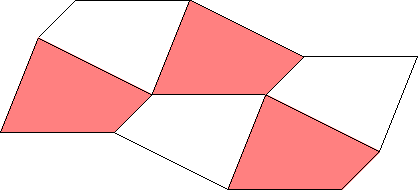
\includegraphics{quadtess.pdf}
  \]
  Now you tessellate the quadrilateral below:
  \[
  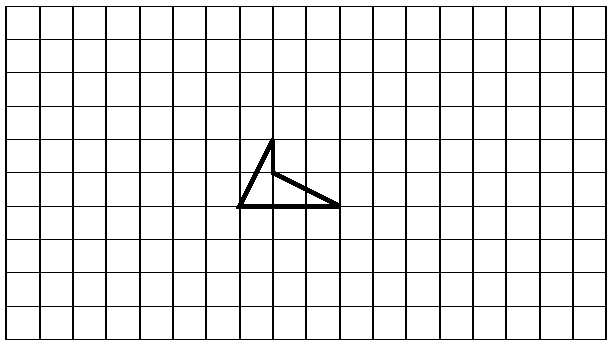
\includegraphics{109exam1_tess.pdf}
  \]
  \textbf{Draw enough so that we can see that your pattern actually
    tessellates the plane.}
\end{question}
\mynewpage

\begin{question}
  Demonstrate how to tile the plane with a 9-gon, now a 10-gon!

  \begin{hint}
    Think about the shape of a comb.
  \end{hint}  
\end{question}
\mynewpage



\begin{question}
  Do you recall, the \textit{most famous theorem of all?}
    \begin{mdframed}[style=OutcomeStyle]\begin{quote}
    The \underline{Pythagorean theorem} says that given a right
    triangle,
    \begin{center}
      \begin{tikzpicture}[geometryDiagrams]
        \coordinate (A) at (0,0);
        \coordinate (B) at (0,3);
        \coordinate (C) at (7,0);
        \tkzDrawSegment (A,B)
        \tkzDrawSegment (A,C)
        \tkzDrawSegment (C,B)
        \tkzLabelSegment[left](A,B){$a$}
        \tkzLabelSegment[below](A,C){$b$}
        \tkzLabelSegment[above right](B,C){$c$}  

        \tkzMarkRightAngle[thin](C,A,B)
        %\tkzLabelAngle[pos=1.2](C,A,B){$?$}

        %% \tkzMarkAngle[size=0.8cm,thin,mark=](A,B,C)
        %% \tkzLabelAngle[pos=.5](A,B,C){$?$}

        %% \tkzMarkAngle[mark=,size=.9,thin](B,C,A)
        %% \tkzLabelAngle[pos=.6](B,C,A){$?$}
        
      \end{tikzpicture}
    \end{center}
    we will always have that
    \[
    a^2 + b^2 = c^2.
    \]
   \end{quote}
    \end{mdframed}
    EXPLAIN (using words, pictures, and so on) how the picture
    below``proves'' the Pythagorean Theorem:
    \[
    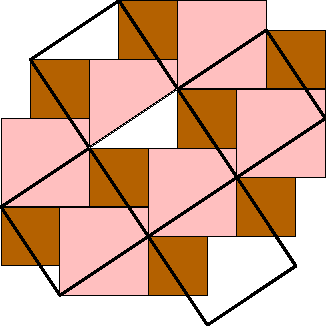
\includegraphics{pbppyth2.pdf}
    \]
    \begin{freeResponse}
      The white triangle is our right triangle. The area of the middle
      overlaid square is $c^2$, the area of the small dark squares is $a^2$,
      and the area of the medium lighter square is $b^2$. Now label all the
      ``parts'' of the large overlaid square:
      \[
      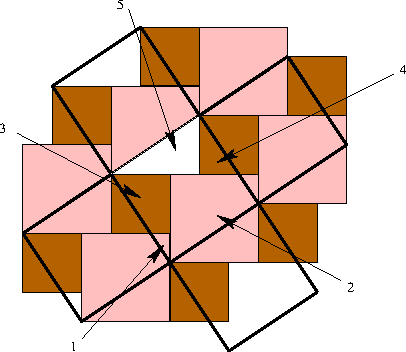
\includegraphics{pbppyth2a.pdf}
      \]
      From the picture we see that
      \begin{align*}
        a^2 &= \{\text{3 and 4}\}\\
        b^2 &= \{\text{1, 2, and 5}\}\\
        c^2 &= \{\text{1, 2, 3, 4, and 5}\}
      \end{align*}
      Hence
      \[
      c^2 = a^2 + b^2
      \]
      Since we can always put two squares together in this pattern, this
      proof will work for any right triangle.
    \end{freeResponse}
\end{question}



\end{document}
